%\VignetteIndexEntry{RCyjs}
%\VignettePackage{RCyjs}
%\VignetteEngine{utils::Sweave}

\documentclass{article}

\RequirePackage{/Library/Frameworks/R.framework/Versions/3.1/Resources/library/BiocStyle/resources/latex/Bioconductor}

\AtBeginDocument{\bibliographystyle{/Library/Frameworks/R.framework/Versions/3.1/Resources/library/BiocStyle/resources/latex/unsrturl}}
\newcommand{\exitem}[3]{\item \texttt{\textbackslash#1\{#2\}} #3 \csname#1\endcsname{#2}.}
\title{RCyjs: using Cytoscape.js from an R session}
\author{Paul Shannon}

\usepackage{/Library/Frameworks/R.framework/Resources/share/texmf/tex/latex/Sweave}
\begin{document}

\maketitle

\tableofcontents

\section{Introduction}

\Biocpkg{RCyjs} is a \Biocpkg{BrowserViz} subclass providing interactive access to Cytoscape.js running in your
browser from an R session.  Cytoscape.js \url{http://js.cytoscape.org} provides full-featured network visualization in an HTML5
browser window.  This web-based implementation is related to, and can exchange data with the
desktop version of Cytoscape: \url{http://cytoscape.org}.    See the \Biocpkg{BrowserViz} vignette for
a description of the websocket and JSON techniques used here to connect your R session to your browser.

\section{Simple Example}

\Biocpkg{RCyjs} provides a utility function which creates a small 3-node, 3-edge graphNEL (see \Biocpkg{graph})
with some attributes assigned to the nodes and edges:

\begin{Schunk}
\begin{Sinput}
> library(RCyjs)
> g <- simpleDemoGraph()
> noaNames(g)
\end{Sinput}
\begin{Soutput}
[1] "type"  "lfc"   "label" "count"
\end{Soutput}
\begin{Sinput}
> edaNames(g)
\end{Sinput}
\begin{Soutput}
[1] "edgeType" "score"    "misc"    
\end{Soutput}
\begin{Sinput}
> noa(g, "type")
\end{Sinput}
\begin{Soutput}
                     A                      B                      C 
              "kinase" "transcription factor"         "glycoprotein" 
\end{Soutput}
\begin{Sinput}
> noa(g, "lfc")
\end{Sinput}
\begin{Soutput}
 A  B  C 
-3  0  3 
\end{Soutput}
\begin{Sinput}
> eda(g, "edgeType")
\end{Sinput}
\begin{Soutput}
               A|B                B|C                C|A 
  "phosphorylates" "synthetic lethal"        "undefined" 
\end{Soutput}
\begin{Sinput}
> eda(g, "score")
\end{Sinput}
\begin{Soutput}
A|B B|C C|A 
 35 -12   0 
\end{Soutput}
\end{Schunk}

Send this graph to your browser and render it with all default settings (including faint edges connecting the nodes):
\begin{Schunk}
\begin{Sinput}
> g <- simpleDemoGraph()
> rcy <- RCyjs(portRange=9047:9067, quiet=TRUE, graph=g);
> title <- "simple graph"
> setBrowserWindowTitle(rcy, title)
\end{Sinput}
\begin{Soutput}
[1] "simple graph"
\end{Soutput}
\end{Schunk}

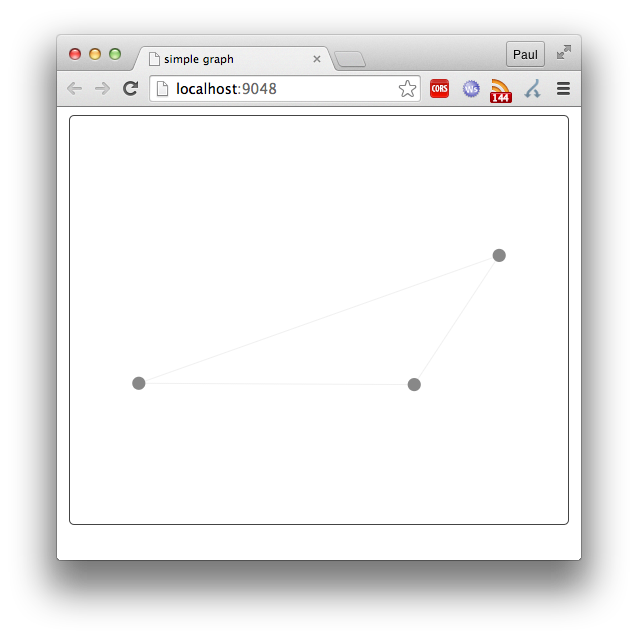
\includegraphics[width=0.8\textwidth]{fig0.png}

In network visualization we commonly use edge and node attributes to control visual appearance.
For instance, an edgeType of ``phosphorylates'' could be rendered in green, and ``regulates'' in black.
Node size can reflect expression levels or population size.  Node borders can indicate abnormal modifications.
This process, and the rules that govern it, go by the name of ``visual mapping''.  

Before discussing and illustrating the use of these rules, let us first see how to set default 
visual properties which apply to all parts of the graph.  For instance: make all nodes round, with
white interior, a thin black border, 50 pixels in diameter, connected by black edges (lines) which
have no terminal decoration (that is, no arrows at the ends of the edges).  Note that \emph{redraw}
must be called to \emph{apply} the currently specified rules.  First we define some useful colors:

\begin{Schunk}
\begin{Sinput}
> green <- "rgb(0,255,0)"
> white <- "rgb(255,255,255)"
> red <- "rgb(255,0,0)"
> blue <- "rgb(0,0,255)"
> black <- "rgb(0,0,0)"
> darkGreen <- "rgb(0,200,0)"
> darkerGreen <- "rgb(0,120,0)"
> darkRed <- "rgb(221,0,0)"
> darkerRed <- "rgb(170,0,0)"
> purple <- "rgb(221,221,0)"
> darkBlue <- "rgb(0,0,170)"
> darkerBlue <- "rgb(0,0,136)"
> lightGray="rgb(230,230,230)"
> 
\end{Sinput}
\end{Schunk}

\begin{Schunk}
\begin{Sinput}
> setDefaultNodeShape(rcy, "ellipse")
> setNodeLabelRule(rcy, "label")  # we DO want a different label on each node.  this rule ensures that
> setDefaultNodeSize(rcy, 70)
> setDefaultNodeColor(rcy, "white")
> setDefaultNodeBorderColor(rcy, "black")
\end{Sinput}
\begin{Soutput}
[1] ""
\end{Soutput}
\begin{Sinput}
> setDefaultNodeBorderWidth(rcy, 1)
\end{Sinput}
\begin{Soutput}
[1] ""
\end{Soutput}
\begin{Sinput}
> setDefaultEdgeColor(rcy, blue)
> setNodeLabelAlignment(rcy, "center", "center");
> layout(rcy, "circle")
\end{Sinput}
\begin{Soutput}
[1] ""
\end{Soutput}
\begin{Sinput}
> fitContent(rcy)
> setZoom(rcy, 0.75 * getZoom(rcy))
> setDefaultEdgeSourceArrowShape(rcy, "tee")
> setDefaultEdgeTargetArrowShape(rcy, "triangle")
> setDefaultEdgeSourceArrowColor(rcy, blue)
> setDefaultEdgeTargetArrowColor(rcy, blue)
> redraw(rcy)
\end{Sinput}
\end{Schunk}

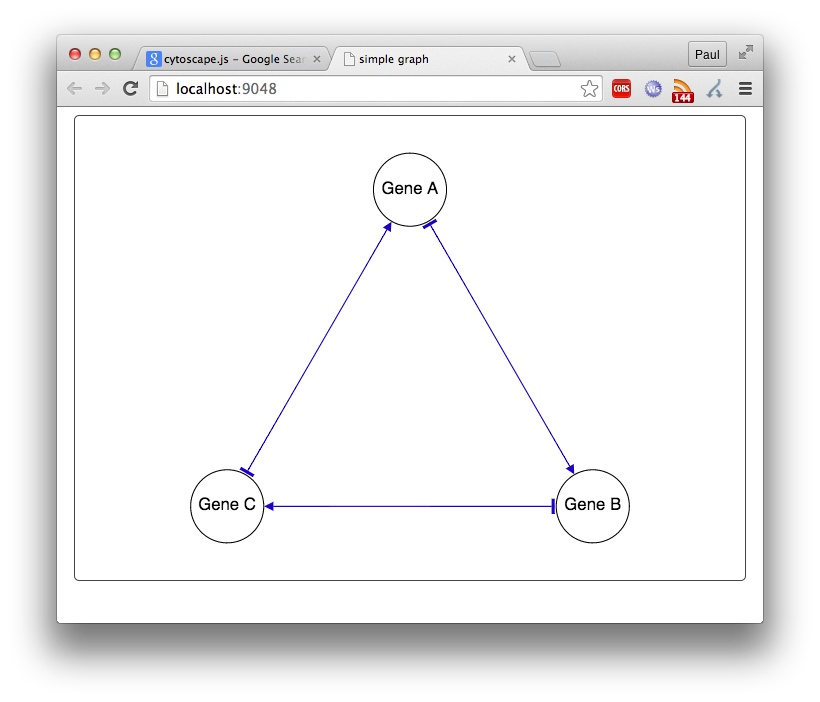
\includegraphics[width=0.8\textwidth]{fig1.png}
Node colors are perhaps the first part of the network you may want to render as a function of node attributes.
We will use ``lfc'' (for log-fold change) frequently used as a measure of microarray expression ratios.
We use the ``interpolate'' mode; intermediate values are interpolated from the control.points and their
associated colors.   We use \emph{edgeType} to control edge color, in ``lookup'' mode.  Note that not all
rules have both modes.  Node shape, for instance, offers only discrete options (ellipse, rectangle, etc.),
and no mode need be specified.
\begin{Schunk}
\begin{Sinput}
> noa(g, "lfc")
\end{Sinput}
\begin{Soutput}
 A  B  C 
-3  0  3 
\end{Soutput}
\begin{Sinput}
> setNodeColorRule(rcy, "lfc", c(-5, 0, 5), c(green, white, red), mode="interpolate")
> setEdgeColorRule(rcy, "edgeType",
+                  c("phosphorylates", "synthetic lethal", "undefined"),
+                  c(red, green, blue), mode="lookup")
> redraw(rcy)
\end{Sinput}
\end{Schunk}
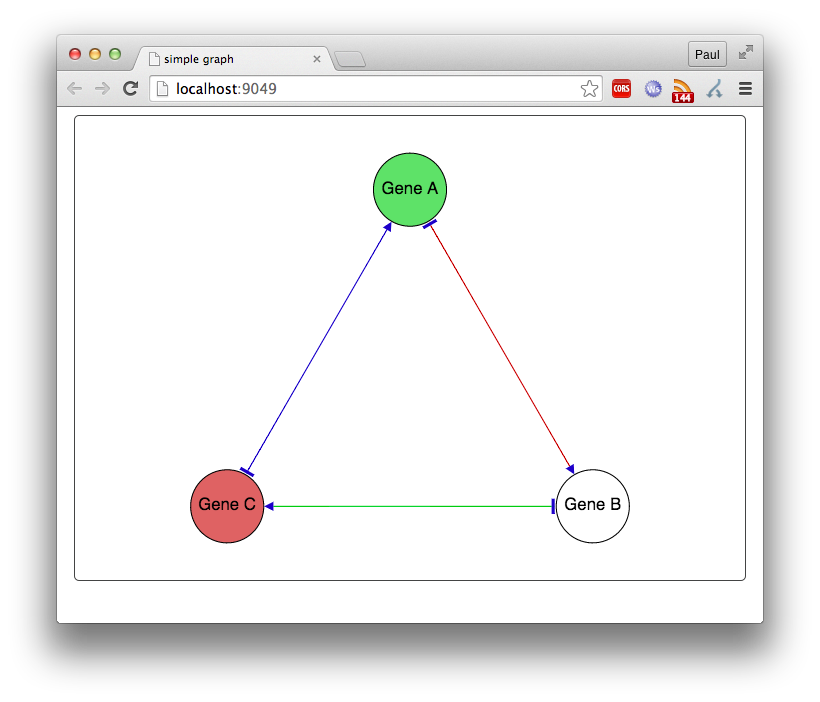
\includegraphics[width=0.8\textwidth]{fig2.png}

\section{Larger Example: Hypoxia Induction Network}

The \Biocpkg{RefNet}) and \Biocpkg{PSICQUIC} packages offer programmatic access to curated molecular (mostly protein) interactions.
Among the interactions we have collected and offer through \Biocpkg{RefNet} is one extracted from a Pouyssegur et al, 2006:

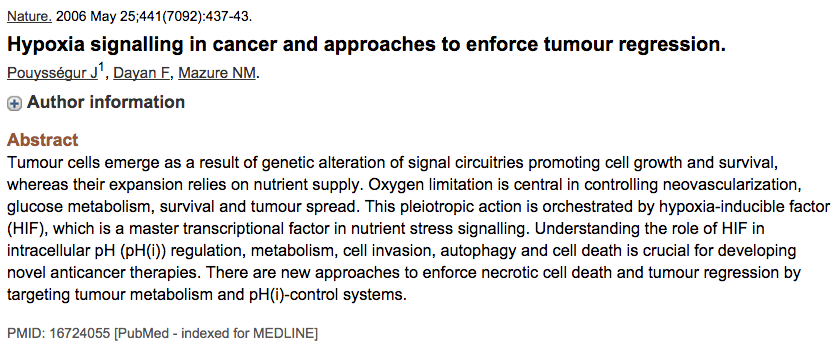
\includegraphics[width=0.8\textwidth]{abstract.png}

In this section, we load a \Biocpkg{RefNet} data.frame describing the interactions reported in that paper, and display then using
\Biocpkg{RCyjs}.  First we define a utility method for createing a \emph{graphNEL} from a RefNet data.frame:

\begin{Schunk}
\begin{Sinput}
> refnetToGraphNEL <- function(tbl)
+ {
+   g = new ("graphNEL", edgemode="directed")
+   nodeDataDefaults(g, attr="type") <- "undefined"
+   nodeDataDefaults(g, attr="label") <- "default node label"
+   nodeDataDefaults(g, attr="expression") <-  1.0
+   nodeDataDefaults(g, attr="gistic") <-  0
+   nodeDataDefaults(g, attr="mutation") <-  "none"
+   edgeDataDefaults(g, attr="edgeType") <- "undefined"
+   edgeDataDefaults(g, attr= "pubmedID") <- ""
+   all.nodes <- sort(unique(c(tbl$A, tbl$B)))
+   g = graph::addNode (all.nodes, g)
+   nodeData (g, all.nodes, "label") = all.nodes
+   g = graph::addEdge (tbl$A, tbl$B, g)
+   edgeData (g, tbl$A, tbl$B, "edgeType") = tbl$type
+   g
+   }
\end{Sinput}
\end{Schunk}

Load \Biocpkg{RefNet}, request the interactions described in the paper, convert them to a graphNEL:
\begin{Schunk}
\begin{Sinput}
> library(org.Hs.eg.db)
> library(RefNet)
> refnet <- RefNet();
\end{Sinput}
\begin{Soutput}
[1] initializing PSICQUIC...
[1] initializing RefNet from AnnotationHub...
[1] RefNet ready.
\end{Soutput}
\begin{Sinput}
> tbl.hypoxia <- interactions(refnet,provider="hypoxiaSignaling-2006")
> g.hypoxia <- refnetToGraphNEL(tbl.hypoxia)
\end{Sinput}
\end{Schunk}
Most of the the nodes in the graph are genes, and some are biological processes.  The network display will
be easier to grasp if these two categories are rendered differently.   Use the \Biocpkg{org.Hs.eg.db}:
any node name mentioned there will be a gene, all others will be processes.

\begin{Schunk}
\begin{Sinput}
> all.nodes <- nodes(g.hypoxia)
> gene.nodes <- intersect(all.nodes, keys(org.Hs.egSYMBOL2EG))
> process.nodes <- setdiff(all.nodes, gene.nodes)
> nodeData(g.hypoxia, gene.nodes, attr="type") <- "gene"
> nodeData(g.hypoxia, process.nodes, attr="type") <- "process"
\end{Sinput}
\end{Schunk}

Create and display the network, using the first open port between 9047 and 9067 to connect to your
default browser.  Set some default rendering rules, and the browser window title.  The nodes
will be arranged randomly on the browser canvas.

\begin{Schunk}
\begin{Sinput}
> rcy <- RCyjs(portRange=9047:9067, quiet=TRUE, graph=g.hypoxia);
> setBackgroundColor(rcy, lightGray)
> setDefaultNodeSize(rcy, 60)
> setDefaultNodeColor(rcy, white)
> setDefaultNodeBorderColor(rcy, black)
\end{Sinput}
\begin{Soutput}
[1] ""
\end{Soutput}
\begin{Sinput}
> setDefaultNodeBorderWidth(rcy, 3)
\end{Sinput}
\begin{Soutput}
[1] ""
\end{Soutput}
\begin{Sinput}
> setNodeLabelRule(rcy, "label");
> setNodeShapeRule(rcy, "type", c("gene", "process"), c("ellipse", "roundrectangle"))
> redraw(rcy)
> title <- "Hypoxia Signaling: Pouyssegur 2006"
> setBrowserWindowTitle(rcy, title)
\end{Sinput}
\begin{Soutput}
[1] "Hypoxia Signaling: Pouyssegur 2006"
\end{Soutput}
\end{Schunk}

Cytoscape.js provides several automated layout algorithms, but optimal layout nearly always involves 
at least some manual placement of nodes as well.  One such layout is included in the package. 
Recreate it by loading the file into which it was saved, and applying it.  Then size the
full network to occupy most of the browser canvas.

\begin{Schunk}
\begin{Sinput}
> saved.layout.file <- system.file(package="RCyjs", "extdata", "hypoxiaLayout.RData")
> stopifnot(file.exists(saved.layout.file))
> restoreLayout(rcy, saved.layout.file)
> fitContent(rcy)
> setZoom(rcy, 0.9 *getZoom(rcy))
\end{Sinput}
\end{Schunk}
Use the interaction type, specified in the \Biocpkg{RefNet} data.frame, and copied into the graphNEL as the 
edge attribute ``edgeType'' to control the color of the displayed edges.  Use this same information to
control what shape, if any, is displayed to ``decorate'' the edge:  a triangle indicates a positive 
effect of the upstream node on the downstream node; a ``tee'' indicates a negative effect.   Finally,
after specifying these rules, redraw the network and the rules are applied


\begin{Schunk}
\begin{Sinput}
> edgeColors <- list(activates = darkerGreen,
+                    inhibits = darkRed,
+                    inactivates = darkRed,
+                    hydroxylates = black,
+                    "TF cofactor" = darkBlue,
+                    "TF binding" = darkBlue,
+                    hydroxylated = black,
+                    stabilizes.mrna = darkerBlue,
+                    preserves = darkGreen,
+                    proteolyzes = darkRed)
> setEdgeColorRule(rcy, "edgeType", names(edgeColors), as.character(edgeColors), mode="lookup")
> setEdgeTargetArrowColorRule(rcy, "edgeType", names(edgeColors), as.character(edgeColors),
+                             mode="lookup")
\end{Sinput}
\end{Schunk}

edgeTargetShapes <- list(activates = "triangle",
                         inhibits = "tee",
                         inactivates = "tee",
                         hydroxylates = "triangle",
                         "TF cofactor" = "none",
                         "TF binding" = "triangle",
                         hydroxylated = "none",
                         stabilizes.mrna = "triangle",
                         preserves = "triangle",
                         proteolyzes = "triangle")

setEdgeTargetArrowShapeRule(rcy, "edgeType", names(edgeTargetShapes), as.character(edgeTargetShapes))

redraw(rcy)
Sys.sleep(3)   # allow the redraw to complete before ending


  
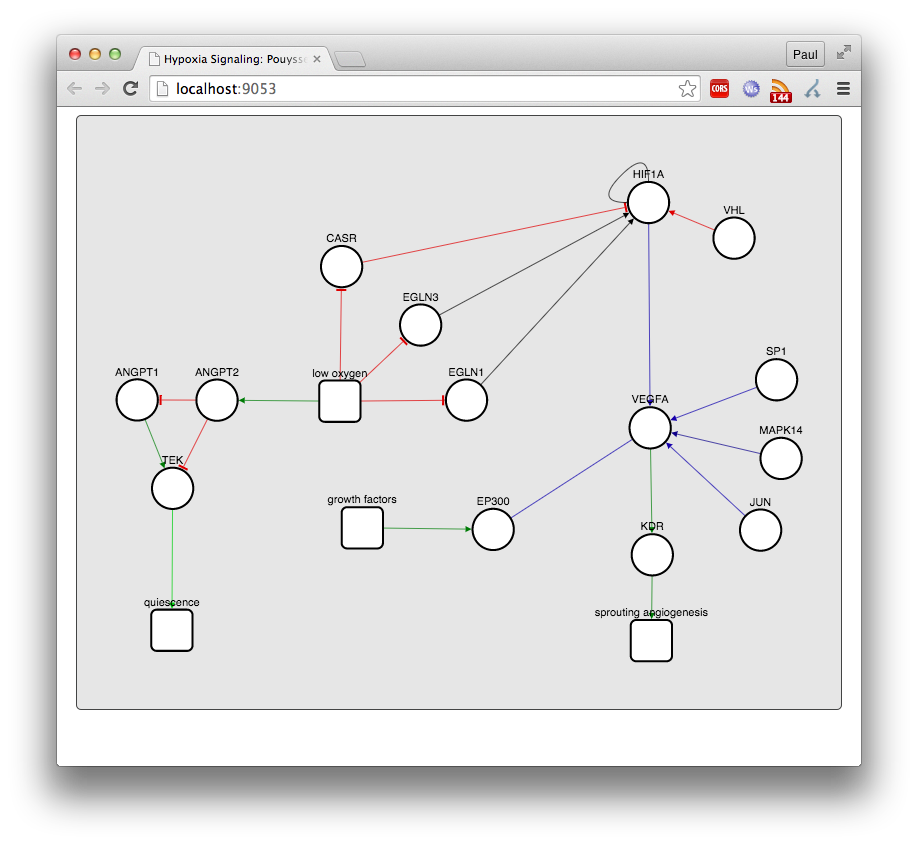
\includegraphics[width=0.8\textwidth]{hypoxiaNetwork.png}

\end{document}
